\chapter{Analysis, Design, and Implementation of Analytical Information Systems (OLAP)}

Having established the formalism for systems that capture the transactional state of a domain, we now turn our attention to systems designed to analyze the temporal evolution of that state. Online Analytical Processing (OLAP) systems are not concerned with recording atomic operations, but with the aggregation, pattern discovery, and modeling of large-scale historical data. This is the domain of Business Intelligence (BI).

\section{Problems and Challenges in Business Intelligence}
The transition from data collection to the extraction of actionable knowledge is nontrivial. It requires a fundamentally different architecture and a reframing of modeling, moving from normalization for write efficiency to denormalization for aggregate read efficiency.

\subsection{Basic Concepts}
\begin{definition}[Business Intelligence (BI)]
Business Intelligence is a paradigm that encompasses a set of theories, methodologies, architectures, and technologies that transform raw data into meaningful and useful information and knowledge for purposes of analysis and strategic decision-making in an organization. While OLTP systems answer the question, "What is the current state of the system?", BI systems answer, "What are the trends and patterns emerging from the history of the system's states?".
\end{definition}

\begin{definition}[Online Analytical Processing (OLAP)]
OLAP is the underlying technology that enables fast, interactive, multidimensional analysis of large volumes of data. An OLAP "cube" is the conceptual data structure that allows this analysis, representing data through \textbf{dimensions} (axes of analysis, e.g., time, geography, product) and \textbf{measures} (numeric values to be aggregated, e.g., sales, revenue).
\end{definition}

The fundamental challenge is that data generated by OLTP systems is not structured for analysis. It is highly normalized to minimize redundancy and optimize writes, resulting in complex schemas of dozens or hundreds of tables. A simple analytical query ("What were the total sales by region in the last quarter?") would require a prohibitive number of join operations on these schemas, resulting in unacceptable performance.

\subsection{Canonical BI System Architecture}
To solve this problem, a decoupled architecture is postulated, where operational data is periodically extracted, transformed, and loaded into a central repository optimized for analysis.

\begin{center}
\resizebox{0.9\textwidth}{!}{%
\begin{tikzpicture}[node distance=2.5cm, auto, >=latex']
    \node[draw, rectangle, rounded corners] (sources) {Data Sources (OLTP, Files, etc.)};
    \node[draw, rectangle, rounded corners, right of=sources, xshift=3.2cm] (etl) {ETL Process};
    \node[draw, cylinder, shape border rotate=90, aspect=0.5, right of=etl, xshift=2.5cm] (dwh) {Data Warehouse (DWH)};
    \node[draw, cylinder, shape border rotate=90, aspect=0.5, above of=dwh, yshift=-0.5cm] (dm1) {Data Mart 1};
    \node[draw, cylinder, shape border rotate=90, aspect=0.5, below of=dwh, yshift=0.5cm] (dm2) {Data Mart N};
    \node[draw, rectangle, rounded corners, right of=dwh, xshift=3.5cm] (analysis) {Analysis Tools (OLAP, Reporting)};
    
    \path[->] (sources) edge node[midway, above, font=\small] {Extract} (etl);
    \path[->] (etl) edge node[midway, above, font=\small] {Load} (dwh);
    \path[->] (dwh) edge (dm1);
    \path[->] (dwh) edge (dm2);
    \path[->] (dm1) edge (analysis);
    \path[->] (dm2) edge (analysis);
    \path[->] (dwh) edge [bend left=45] (analysis);
\end{tikzpicture}%
}
\end{center}

\begin{description}
    \item[Data Sources:] The OLTP systems, spreadsheets, server logs, etc., that generate operational data.
    \item[ETL (Extract, Transform, Load) Process:] The core of the system.
    \begin{itemize}
        \item \textbf{Extract:} Obtaining the data from the sources.
        \item \textbf{Transform:} The most complex phase. It includes data cleansing (handling nulls, correcting errors), integration (unifying data from multiple sources), and denormalization to create a \textbf{dimensional model}.
        \item \textbf{Load:} Inserting the transformed data into the Data Warehouse.
    \end{itemize}
    \item[Data Warehouse (DWH):] A central, integrated, historical, and non-volatile repository of data. It is the "single source of truth" for the entire organization.
    \item[Data Marts:] Subsets of the DWH, oriented towards a specific business area (e.g., Sales, Finance), to simplify access and improve performance.
\end{description}

\subsection{What is a Business Model?}
Before any data can be analyzed, it is imperative to formally understand the domain that generates it. A business model is an abstract description of how an organization creates, delivers, and captures value. It is not merely an economic concept but a system of interconnected processes.

\subsection{What is a Business Model?}
Before any data can be analyzed, it is imperative to formally understand the domain that generates it. A business model is a conceptual blueprint that describes the rationale of how an organization creates, delivers, and captures value. While not a rigid mathematical formula, it can be deconstructed into a set of core, interconnected components. The most widely accepted formal framework for this is the Business Model Canvas, which defines a business model through nine building blocks:

\begin{description}
    \item[Customer Segments] The distinct groups of people or organizations an enterprise aims to reach and serve.
    \item[Value Propositions] The bundle of products and services that create value for a specific Customer Segment. It is the reason why customers turn to one company over another.
    \item[Channels] Describes how a company communicates with and reaches its Customer Segments to deliver a Value Proposition.
    \item[Customer Relationships] The types of relationships a company establishes with specific Customer Segments (e.g., transactional, long-term, automated).
    \item[Revenue Streams] The cash a company generates from each Customer Segment. It represents the captured value.
    \item[Key Resources] The most important assets required to make the business model work (e.g., physical, intellectual, human, financial).
    \item[Key Activities] The most important actions a company must perform to operate successfully (e.g., production, problem-solving, platform management).
    \item[Key Partnerships] The network of suppliers and partners that make the business model work.
    \item[Cost Structure] All costs incurred to operate a business model.
\end{description}

The purpose of a business intelligence system is to quantify the performance and interplay of these nine blocks. For example, a BI system can measure the profitability of different \textbf{Customer Segments}, the effectiveness of various \textbf{Channels}, or the cost-efficiency of \textbf{Key Activities}. The BI system's data model must be designed to capture the metrics that illuminate these fundamental components.

\subsection{Questions for Building a Business Model and BPMN}
The analysis of a business model revolves around a series of fundamental questions: Who are our customers? What value do we deliver to them? Through which channels? What key activities do our processes require?
To formally model the business processes ($\mathcal{P}$), a graphical standard called \textbf{Business Process Model and Notation (BPMN)} is used. BPMN is a visual language that allows for the specification of workflows in a manner analogous to how a flowchart specifies an algorithm.

Its main elements are:
\begin{itemize}
    \item \textbf{Events:} Circles representing something that "happens" (e.g., order initiated, payment received).
    \item \textbf{Activities:} Rounded-corner rectangles representing work that is "done" (e.g., check inventory, ship product).
    \item \textbf{Gateways:} Diamonds that control the divergence and convergence of the flow (e.g., decisions, parallel flows).
    \item \textbf{Sequence Flows:} Arrows that connect the preceding elements.
\end{itemize}
\begin{figure}[h]
    \centering
    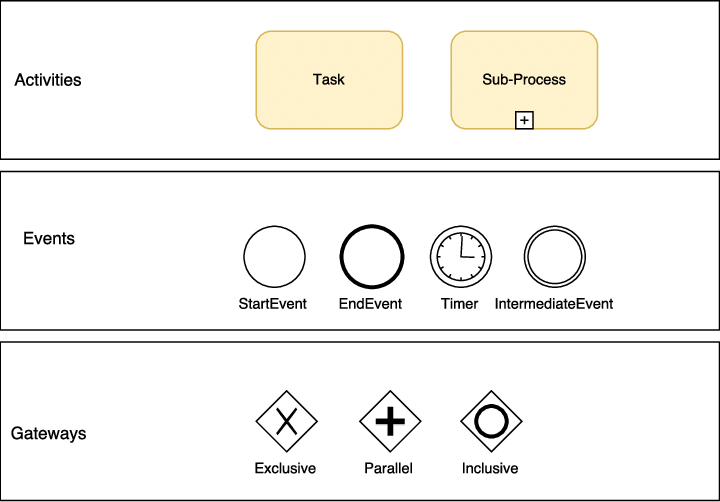
\includegraphics[width=0.5\linewidth]{Notation.png}
    \caption{BPMN extended notation}
    \label{fig:placeholder}
\end{figure}
Modeling in BPMN is the first step in identifying what must be measured in an organization.

\subsection{Establishing Key Performance Indicators (KPIs)}
Once the business processes are formally defined, it is necessary to quantify their performance.
\begin{definition}[Key Performance Indicator (KPI)]
A Key Performance Indicator (KPI) is a function $f: S \to \mathbb{R}$, where $S$ is the state space of a business process, which maps the process state to a quantifiable numeric value. This value is compared against a predefined target to evaluate performance. A KPI must be:
\begin{itemize}
    \item \textbf{Quantifiable:} Measurable in a numerical way.
    \item \textbf{Actionable:} Its value must be able to be influenced by the organization's actions.
    \item \textbf{Strategic:} It must be directly aligned with a business objective.
\end{itemize}
\end{definition}
\textit{Examples:} Sales Conversion Rate ( (Number of Sales / Number of Leads) $\times$ 100), Customer Acquisition Cost (Total Marketing Cost / Number of New Customers), Order Cycle Time.

The selection of the correct KPIs is the culmination of the requirements analysis in a business intelligence project. These KPIs dictate which measures and dimensions must be modeled in the OLAP cube, what data must be extracted by the ETL, and ultimately, what knowledge can be extracted from the system.

\section{Analysis and Design of the Data Warehouse}
The transition from the OLTP domain to the OLAP domain is not merely a change in application; it is a fundamental paradigm shift in the philosophy of data modeling. The highly normalized schemas (3NF/BCNF), which are masterpieces of efficiency for transactional integrity and the minimization of redundancy, become an insurmountable bottleneck for the complex, large-scale aggregate queries that define business intelligence. The objective is no longer the optimization of atomic write operations, but the optimization of massive, aggregate read operations. This necessitates a new formalism: multidimensional modeling.

\subsection{The Multidimensional Modeling Paradigm}
Multidimensional modeling is a design methodology that structures data not around atomic entities and their relationships, but around the continuous processes of a business and the discrete, numerical measurements (events) that these processes generate. It provides an intuitive, high-performance framework for analytical queries by abstracting data into a structure analogous to a geometric hypercube.

\begin{definition}[Multidimensional Model]
A multidimensional model is a data model that organizes data in a logical hypercube, or "cube". This n-dimensional structure consists of two fundamental and orthogonal types of components:
\begin{itemize}
    \item \textbf{Facts:} The numerical measurements that correspond to a specific event within a business process. These form the quantitative body of the cube.
    \item \textbf{Dimensions:} The categorical context that defines the coordinate axes of the hypercube. They provide the "who, what, where, when, why" context for the facts.
\end{itemize}
An analytical query, therefore, is no longer a complex traversal of a graph of normalized tables, but rather a "slice" or an aggregation across a sub-volume of this hypercube.
\end{definition}

\subsection{The Axiomatic Components: Facts and Dimensions}
The clean, orthogonal separation between facts (what is measured) and dimensions (the context of measurement) is the foundational axiom of dimensional modeling.

\subsubsection{Fact Tables and Their Types}
A fact represents a specific, quantifiable event. These events are stored in a central \textbf{fact table}. Every row in this table corresponds to a discrete measurement at a specific point in the n-dimensional space defined by the dimensions. Fact tables are the gravitational center of the model.

\begin{description}
    \item[Granularity:] The single most important concept in dimensional modeling. The \textbf{grain} of the fact table is a formal declaration of what a single row represents (e.g., "one individual product line item on a customer's sales receipt"). Every design decision flows from this declaration.
    \item[Measures:] The numerical attributes that quantify the event. They are classified by their additivity: \textbf{fully additive} (e.g., `quantity\_sold`), \textbf{semi-additive} (e.g., inventory levels, which are not additive across time), and \textbf{non-additive} (e.g., ratios, which must be computed from additive components).
\end{description}

There are three canonical types of fact tables, distinguished by how they record measurements over time:
\begin{description}
    \item[Transactional Fact Tables] This is the most common and fundamental type. Each row corresponds to a single event at a single point in time, representing an instantaneous measurement. The table grows by continuously appending new rows as events occur. The grain is typically fine-grained, capturing the most atomic level of a business process. The `Fact\_Sales` example, where each row represents one line item on one receipt, is a classic transactional fact table. This structure is the most flexible and detailed, allowing for analysis across any time period by aggregating the discrete events.

    \item[Periodic Snapshot Fact Tables] Each row summarizes the state of a subject over a specific, uniform period of time (e.g., a day, a week, a month). This design is ideal for analyzing performance over time and for processes that do not have discrete events, such as account balances. The grain is the period itself (e.g., "one row per customer per month"). For example, a `Fact\_Account\_Monthly\_Snapshot` would have one row per customer per month, recording measures like `end\_of\_month\_balance`, `total\_deposits`, and `total\_withdrawals` for that period. This structure is less sparse than a transactional table but is less flexible for analyzing arbitrary time intervals.

    \item[Accumulating Snapshot Fact Tables] Each row represents the entire lifecycle of a well-defined process that has a clear beginning and end. The table has multiple date columns, each corresponding to a major milestone in the process. The row is visited and updated as the process progresses through its stages. For example, a `Fact\_Order\_Lifecycle` table would have one row per order, with columns for `date\_placed`, `date\_shipped`, `date\_delivered`, and measures like `days\_to\_ship` (calculated as `date\_shipped` - `date\_placed`). This model is excellent for analyzing the latency or duration between milestones in a process, a type of analysis known as pipeline or funnel analysis.
\end{description}

\subsubsection{Dimension Tables and Advanced Concepts}
A dimension represents the rich, textual context of a measurement. They are stored in "wide", denormalized \textbf{dimension tables}.
\begin{itemize}
    \item \textbf{Surrogate Keys:} The primary key of a dimension table must be a system-generated, sequentially assigned integer known as a \textbf{surrogate key}. This decouples the data warehouse from the operational system's keys and is essential for tracking historical changes.
    \item \textbf{Descriptive Attributes:} A dimension table is typically "wide" and "flat", containing a large number of denormalized, textual attributes for query filtering and grouping.
    \item \textbf{Hierarchies:} Attributes within a dimension are organized into fixed-depth hierarchies (e.g., `Product` $\to$ `Brand` $\to$ `Category`), which define the formal paths for aggregation (drilling and rolling up).
\end{itemize}

\begin{description}
    \item[Conformed Dimensions] A \textbf{conformed dimension} is a dimension that is managed once in the ETL system and is shared, with identical structure and content, across multiple fact tables or data marts. For example, a single, master `Dim\_Date` table can be used by `Fact\_Sales`, `Fact\_Inventory`, and `Fact\_Shipments`. The use of conformed dimensions is the cornerstone of an integrated, enterprise-wide data warehouse, as it allows for the seamless combination and comparison of metrics from different business processes. It establishes a common, shared business vocabulary, ensuring that "product" means the same thing to the sales department and the inventory department.

    \item[Slowly Changing Dimensions (SCDs)] A critical problem in data warehousing is how to handle changes to dimensional attributes over time (e.g., a customer moves to a new city, a product is reassigned to a new category). Several formal techniques exist to manage this historical tracking, ensuring that analysis of historical facts remains accurate.
    \begin{itemize}
        \item \textbf{Type 1 (Overwrite):} The simplest approach. The old attribute value is overwritten with the new value. No history is preserved. This technique is appropriate only for correcting errors and should never be used for actual changes in the domain, as it corrupts the historical record.
        \item \textbf{Type 2 (Add a New Row):} This is the most common, powerful, and fundamental method for historical tracking. When a significant attribute changes, a new row is added to the dimension table for the same entity, with a new surrogate key. The old and new rows are distinguished by versioning columns (e.g., `start\_date`, `end\_date`, `is\_current\_flag`). This technique perfectly preserves all historical context, allowing facts to be correctly associated with the dimensional attributes as they existed at the time of the event. For instance, sales made by a customer in California are forever tied to the California record, even after the customer moves and a new record is created for their new address.
        \item \textbf{Type 3 (Add a New Attribute):} A new attribute is added to the dimension table to store a limited amount of historical information. For example, to track a customer's previous state, one might add a `previous\_state` column alongside the `current\_state` column. This method can only track one historical change and is rarely used as it is not a general solution.
    \end{itemize}
\end{description}

\begin{center}
\begin{tikzpicture}[
    node distance=3.5cm and 3cm, % y-distance and x-distance
    auto,
    >=latex',
    fact/.style={draw, rectangle, rounded corners, fill=blue!10, text width=3.5cm, align=center, minimum height=2cm, font=\small},
    dim/.style={draw, rectangle, rounded corners, fill=green!10, text width=3.5cm, align=center, font=\small}
]
    % Node placement
    \node[fact] (fact) {\textbf{Fact\_Sales} \\ \hline \underline{date\_key} (FK) \\ \underline{product\_key} (FK) \\ \underline{store\_key} (FK) \\ \textit{quantity\_sold} \\ \textit{revenue}};
    \node[dim, above=of fact] (time) {\textbf{Dim\_Date} \\ \hline \underline{date\_key} \\ full\_date \\ month\_name \\ year};
    \node[dim, left=of fact] (product) {\textbf{Dim\_Product} \\ \hline \underline{product\_key} \\ product\_name \\ brand \\ category};
    \node[dim, right=of fact] (store) {\textbf{Dim\_Store} \\ \hline \underline{store\_key} \\ store\_name \\ city \\ state};

    % Edge placement
    \path[->] (time) edge (fact);
    \path[->] (product) edge (fact);
    \path[->] (store) edge (fact);
\end{tikzpicture}
\captionof{figure}{Diagram of a Star Schema. Note the single join path from each dimension to the fact table.}
\end{center}

\subsection{The Star Schema: A Radically Denormalized Model}
The Star Schema is the most fundamental, elegant, and widely used structure in dimensional modeling. It is the purest implementation of the fact-dimension dichotomy, consisting of a central fact table connected directly to a set of surrounding dimension tables. Its Entity-Relationship diagram unambiguously resembles a star, with the highly normalized fact table at its center and the denormalized dimension tables radiating outwards.

The defining characteristic of the Star Schema is its radical denormalization. Each dimension is a single, wide table containing all of its descriptive attributes, even if this introduces significant redundancy. For example, the `Dim\_Product` table would repeat the `category` name and `department` name for every single product within that category and department. This is not a design flaw; it is the core feature and a deliberate trade-off. By pre-joining hierarchical data into a flat structure, the model achieves several critical objectives:
\begin{itemize}
    \item \textbf{Simplicity and Intuitiveness:} The model is exceptionally easy for business users and analysts to understand. The business logic is transparent: metrics are in the central table, and all contexts for slicing and dicing are in the directly connected dimension tables.
    \item \textbf{Query Performance:} This denormalization minimizes the number of joins required for a query to an absolute minimum. A typical analytical query will join the central fact table to one or more dimension tables. As there are no further joins required beyond this first level, the query execution path is simple and predictable. Database query optimizers are highly efficient at handling this specific topology, known as a "star join," often employing specialized algorithms. The reduction in join operations drastically reduces query execution time on large datasets.
    \item \textbf{Analytical Tool Compatibility:} Business Intelligence (BI) and OLAP tools are designed and optimized to work with star schemas. They can automatically detect the fact-dimension relationships, hierarchies, and measures, enabling features like drill-down and drill-up with minimal configuration.
\end{itemize}

\subsection{The Snowflake Schema: A Partially Normalized Model}
The Snowflake Schema is a variation of the star schema where the principle of normalization is selectively reintroduced to the dimension tables. If a dimension contains attributes with low cardinality that form a distinct hierarchy (e.g., a product's brand belongs to a category, which belongs to a department), these are factored out into separate, linked tables, conforming to 3NF. This process of normalizing the dimension tables creates a branching structure that resembles a snowflake.

\begin{center}
\begin{tikzpicture}[
    node distance=2.0cm,
    auto,
    >=latex',
    fact/.style={draw, rectangle, rounded corners, fill=blue!10, text width=2.5cm, align=center, minimum height=1.5cm, font=\scriptsize},
    dim/.style={draw, rectangle, rounded corners, fill=green!10, text width=2.5cm, align=center, font=\scriptsize},
    subdim/.style={draw, rectangle, rounded corners, fill=yellow!10, text width=2.5cm, align=center, font=\scriptsize}
]
    % Node placement
    \node[fact] (fact) {\textbf{Fact\_Sales} \\ \hline \underline{date\_key} \\ \underline{product\_key} \\ \underline{store\_key}};
    \node[dim, left=of fact, xshift=0.2cm] (product) {\textbf{Dim\_Product} \\ \hline \underline{product\_key} \\ product\_name \\ \textit{brand\_key} (FK)};
    \node[subdim, left=of product] (brand) {\textbf{Dim\_Brand} \\ \hline \underline{brand\_key} \\ brand\_name \\ \textit{category\_key} (FK)};
    \node[subdim, below=of brand] (category) {\textbf{Dim\_Category} \\ \hline \underline{category\_key} \\ category\_name};

    \node[dim, right=of fact, xshift=-0.2cm] (store) {\textbf{Dim\_Store} \\ \hline \underline{store\_key} \\ store\_name \\ \textit{city\_key} (FK)};
    \node[subdim, right=of store] (city) {\textbf{Dim\_City} \\ \hline \underline{city\_key} \\ city\_name \\ \textit{state\_key} (FK)};

    % Edge placement
    \path[->] (product) edge (fact);
    \path[->] (store) edge (fact);
    \path[->] (brand) edge (product);
    \path[->] (category) edge (brand);
    \path[->] (city) edge (store);
\end{tikzpicture}
\captionof{figure}{Diagram of a Snowflake Schema. Note the multi-join paths required to traverse dimensional hierarchies.}
\end{center}

\begin{description}
    \item[Advantages:] The primary motivation for this design is the reduction of data redundancy. By normalizing the dimensions, storage space is saved because low-cardinality attributes (like a category name) are stored only once. This also simplifies the maintenance of these attributes; a change to a category's name requires updating a single row in the `Dim\_Category` table, rather than updating every product row associated with that category.
    \item[Disadvantages:] The disadvantages are severe and almost always outweigh the benefits in modern systems. It fundamentally violates the core principle of dimensional modeling by reintroducing complexity into the query path. Queries must now perform additional, often numerous, joins to traverse the normalized hierarchies. This increases query execution time, complicates the SQL that analysts must write, and makes the model far less intuitive for end-users and BI tools, which are optimized for the simple star structure.
\end{description}
\begin{remark}
In modern data warehousing practice, the Star Schema is overwhelmingly preferred. The performance penalty of the additional joins required by a Snowflake Schema is generally considered to far outweigh the marginal benefits of storage savings, which have become less critical with decreasing storage costs and the advent of efficient column-store compression. The simplicity, predictability, and performance of the Star Schema remain paramount for analytical systems. The snowflake schema is often regarded as an anti-pattern or, at best, a niche solution for specific, constrained environments.
\end{remark}

\subsection{The Full Taxonomy of Analytical (OLAP) Operations}
The dimensional model is explicitly designed to support a set of classic analytical query operations. These operations provide a powerful vocabulary for exploring the data cube.
\begin{description}
    \item[Drill-Down / Roll-Up] These are the fundamental operations for navigating dimensional hierarchies. \textbf{Drill-Down} moves from a higher level of aggregation to a lower, more detailed level (e.g., from `Year` to `Quarter`). \textbf{Roll-Up} is the inverse, aggregating from a lower level to a higher one (e.g., from `City` to `State`). These operations correspond to adding or removing attributes from the \texttt{GROUP BY} clause of an SQL query.

    \item[Slice] A slice is an operation that performs a selection on a single dimension of the cube, reducing the n-dimensional cube to a smaller sub-cube. It is conceptually equivalent to filtering the data to a single value for one of its dimensions. For example, in a three-dimensional cube of Sales by (Time, Product, Geography), a slice operation would be to select data only for `Time = 'Q4 2024'`. The result is a two-dimensional plane of data for Products and Geography. This corresponds to a `WHERE` clause on a single dimension's attribute.

    \item[Dice] A dice is an operation that performs a selection on two or more dimensions, defining a smaller sub-cube for analysis. It is equivalent to filtering on multiple dimensions simultaneously. For example, dicing the Sales cube would be to select data for `Time = 'Q4 2024'` AND `Geography = 'North America'`. The result is a smaller cube (in this case, a single vector of sales by Product). This corresponds to a `WHERE` clause with multiple conditions connected by `AND`.

    \item[Pivot] This operation rotates the axes of the cube to provide an alternative presentation of the data, often in a crosstabular report. It does not change the data itself, only its view. For example, a report showing `Regions` as rows and `Product Categories` as columns could be pivoted to show `Product Categories` as rows and `Regions` as columns. This is the functionality provided by pivot tables in spreadsheet software.
\end{sdescription}

\subsection{Practical Example: A Sales Data Mart Design}
Let us formalize the design of a dimensional model for analyzing retail sales, following the canonical four-step process.

\begin{enumerate}
    \item \textbf{Step 1: Select the Business Process.} The process is retail sales. This is the source of our quantitative measurements.
    \item \textbf{Step 2: Declare the Grain.} The grain must be an unambiguous declaration of what a single fact row represents. We declare the grain to be: "An individual product line item on a single customer transaction". This implies we cannot store information that is at a higher level (e.g., the total for the entire receipt) or a lower level (e.g., sub-components of a product).
    \item \textbf{Step 3: Identify the Dimensions.} The dimensions are the "who, what, where, when" context for this grain. For our grain, this yields the dimensions: \texttt{Date}, \texttt{Product}, \texttt{Store}, and \texttt{Customer}.
    \item \textbf{Step 4: Identify the Facts.} The facts are the numerical measures consistent with the grain. For each product line item, we can measure: \texttt{quantity\_sold}, \texttt{unit\_price}, \texttt{extended\_revenue}, \texttt{extended\_cost}.
\end{enumerate}

\noindent This analysis leads directly to the following unambiguous Star Schema:

\noindent\textbf{Fact Table:}
\begin{itemize}
    \item \texttt{Fact\_Sales(\underline{date\_key (FK)}, \underline{product\_key (FK)}, \underline{store\_key (FK)}, \underline{customer\_key (FK)}, quantity\_sold, unit\_price, extended\_revenue, extended\_cost)}
\end{itemize}
\noindent\textbf{Dimension Tables:}
\begin{itemize}
    \item \texttt{Dim\_Date(\underline{date\_key}, full\_date, day\_of\_week, month, quarter, year, is\_holiday)}
    \item \texttt{Dim\_Product(\underline{product\_key}, sku\_id, product\_description, brand, category, department)}
    \item \texttt{Dim\_Store(\underline{store\_key}, store\_name, address, city, state, country, region)}
    \item \texttt{Dim\_Customer(\underline{customer\_key}, customer\_name, gender, income\_level, education\_level)}
\end{itemize}

This schema is robust, efficient, and directly supports queries like "What was the total revenue (\textit{fact}) for the 'Electronics' category (\textit{dimension attribute}) in the 'Western' region (\textit{dimension attribute}) during Q4 (\textit{dimension attribute})?".

If we were forced to snowflake this schema, we might normalize the `Dim\_Product` table. The attributes `brand`, `category`, and `department` form a hierarchy. This would result in the following structure:
\begin{itemize}
    \item \texttt{Dim\_Product(\underline{product\_key}, sku\_id, product\_description, \textit{brand\_key (FK)})}
    \item \texttt{Dim\_Brand(\underline{brand\_key}, brand\_name, \textit{category\_key (FK)})}
    \item \texttt{Dim\_Category(\underline{category\_key}, category\_name, \textit{department\_key (FK)})}
    \item \texttt{Dim\_Department(\underline{department\_key}, department\_name)}
\end{itemize}
A query by department would now require joining four tables instead of one, clearly illustrating the performance degradation inherent in the snowflake design.

\subsection{Physical Design and Performance Optimization for Data Warehouses}
The logical design of a star schema must be complemented by a physical design that ensures high performance on massive data volumes. While the logical model simplifies the query path, the physical implementation determines the actual execution speed.
\begin{description}
    \item[Indexing Strategies] While dimension tables are indexed on their primary (surrogate) keys, the critical indexes in a data warehouse are on the foreign key columns of the fact table. These columns typically have low cardinality relative to the total number of fact rows (e.g., a few hundred stores for billions of sales records). For this data profile, standard B-tree indexes are inefficient. Instead, highly efficient \textbf{bitmap indexes} are used. A bitmap index creates a bit vector for each distinct value in the indexed column, with one bit for each row in the table. This allows for extremely fast logical AND and OR operations on the bit vectors when resolving complex queries involving multiple predicates on different dimensions.

    \item[Partitioning] Fact tables, which can grow to billions or trillions of rows, are almost always physically partitioned. The most common and effective partitioning strategy is by the date dimension (e.g., creating one physical partition per month or quarter). This allows the query optimizer to perform \textbf{partition pruning}—scanning only the physically relevant partitions for a given query (e.g., a query for Q4 sales will ignore the partitions for Q1, Q2, and Q3), dramatically reducing I/O and accelerating performance. Partitioning also simplifies data management, as old partitions can be archived or dropped efficiently without affecting the rest of the table.

    \item[Materialized Views (Aggregates)] To provide near-instantaneous query results for common high-level analytical questions, aggregates can be pre-calculated and stored in physical tables known as materialized views or aggregate tables. For example, a daily sales fact table could be pre-aggregated into a `monthly\_sales\_by\_category` aggregate table. A well-configured query optimizer can then automatically redirect user queries to these aggregates when possible, a technique known as \textbf{query rewriting}. This avoids the costly computation of summing billions of rows at runtime, trading storage space for a massive increase in query speed.
\end{sdescription}